\section{Results}
In the following sections results will be presented for the AMPL implementation and for both of the heuristics. The parameter values used in the runs will also be presented. 

\subsection{AMPL implementation}

Implementing the model in AMPL and running the model in CPLEX 12.5 gives the resulting values for the three objective function components displayed in Table \ref{tab:CPLEX_res}. The weights in equations \ref{objfcn} and \ref{constr:s_min} were set to $L = 2$, $A = 1$, $M =100$ and $N=1$, thus making librarians twice as valuable as assistants and stand ins 100 times more valuable than no shift changes. 

\begin{table}[!h]
\centering
\label{tab:CPLEX_res}
\caption{Results from running the Mathematical Model in CPLEX.}
\begin{tabular}{|l|l|l|}
\hline
\rowcolor{Gray} & \textbf{Min num stand ins (lib,ass)} & \textbf{Solution time} \\ \hline
\cellcolor{Gray} \textbf{Result} & \multicolumn{1}{c|}{(3,0)} & \multicolumn{1}{c|}{19 min} \\
\hline
\end{tabular}
\end{table}

These results can be used as benchmark in the heuristics as CPLEX returns an optimal solution. 

\subsection{Weekly scheduling approach}
As most of the costs are correlated with each other some parameter tuning has been required. The final result of the parameter tuning can be seen in Table \ref{tab:cost_parameters}. Their respective descriptions can be seen in Table \ref{tab:all_costs}. 

\begin{table}[!h]
\centering
\caption{List of all costs used in weekly scheduling approach and their respective values.}
\label{tab:cost_parameters}
\begin{tabular}{|l|l|}
\hline
\rowcolor[HTML]{FD6864} 
\multicolumn{2}{|l|}{\cellcolor{corn} \textbf{Demand costs}} \\ \hline
%\multicolumn{2}{|c|}{\cellcolor[HTML]{FD6864}Demand costs}    \\ \hline
\rowcolor[HTML]{C0C0C0} 
Cost name                                      & Value       \\ \hline
Demand\_few\_ass                        & 350         \\ \hline
Demand\_few\_lib                        & 300         \\ \hline
Demand\_many\_ass                       & 200         \\ \hline
Demand\_many\_lib                       & 40          \\ \hline
Demand\_few\_total                             & 800         \\ \hline
Demand\_many\_total                            & 700         \\ \hline
Demand\_evening\_cost         & 20,000 				\\ \hline
Demand\_PL\_good\_ass        & 1,200            \\ \hline
Demand\_PL\_good\_lib        & 800           \\ \hline
Demand\_PL\_bad\_ass         & 1,200           \\ \hline
Demand\_PL\_bad\_lib         & 1,600             \\ \hline
\rowcolor[HTML]{FD6864} 
\multicolumn{2}{|l|}{\cellcolor{corn} \textbf{PL amount costs}} \\ \hline
\rowcolor[HTML]{C0C0C0} 
Cost name                                      & Value       \\ \hline
PL\_good\_amount                  & 1,000                   \\ \hline
PL\_violate\_amount             & 1,500                  \\ \hline
\rowcolor[HTML]{FD6864} 
\multicolumn{2}{|l|}{\cellcolor{corn} \textbf{Weekend costs}} \\ \hline
\rowcolor[HTML]{C0C0C0} 
Cost name                                      & Value       \\ \hline
HB\_amount                       & 15,000    \\ \hline
No\_weekend                & 5,000                   \\ \hline
\rowcolor[HTML]{FD6864} 
\multicolumn{2}{|l|}{\cellcolor{corn} \textbf{Stand-in costs}} \\ \hline
\rowcolor[HTML]{C0C0C0} 
Cost name                                      & Value       \\ \hline
Stand\_in\_cost                     & 5     \\ \hline
\end{tabular}
\end{table}

Worth noting is that these values are most certainly not optimal as they have mostly been assigned using intuition. However, a few relations were determined by either running some tests or using reason. An example is either if $PL\_good\_cost > Demand\_PL\_good\_ass$ or $PL\_good\_cost > Demand\_PL\_good\_lib$. If so, all workers that can be assigned another PL will be, leaving the library overstaffed with PL workers. The reason is because the net of $-PL\_good\_cost + Demand\_PL\_good\_ass/lib$ will be negative meaning it is a preferable insertion even though the library will be overstaffed.

Table \ref{successful_iter} shows the amount of successful iterations on a run. This run is using the same cost parameters shown in Table \ref{tab:cost_parameters}. 
\begin{table}[!h]
\centering
\caption{Amount of successful iterations}
\label{successful_iter}
\begin{tabular}{|c|c|}
\hline
Successful iterations         & 420      \\ \hline
Iterations (total) & 638      \\ \hline
\%                 & $\sim$66 \\ \hline
\end{tabular}
\end{table}

<<<<<<< HEAD
Based on the same data as in Table \ref{successful_iter} the average stand-in value per iteration can be calculated. It is seen in Table \ref{tab:average_stand_ins}.
\begin{table}[!h]
\centering
\caption{Average stand-in value per iteration}
\label{tab:average_stand_ins}
\begin{tabular}{|c|c|}
\hline
Stand-in value & 105      \\ \hline
Number of iterations         & 420      \\ \hline
Average stand-in value      & 0.25 \\ \hline
\end{tabular}
\end{table}
A librarian is multiplied by a factor two and an assistant is multiplied by a factor one.

Having an average stand-in value of 0.25 means that most of the times no stand-ins are found. About once every fourth or once every eighth iteration was an assistant or librarian found respectively during the run. Table \ref{tab:stand_in_spread} shows statistics of how many stand-ins were found after 420 successful iterations. 
\begin{table}[!h]
\centering
\caption{Amount of stand-ins found after 420 successful iterations.}
\label{tab:stand_in_spread}
\begin{tabular}{|c|c|}
\hline
\rowcolor[HTML]{D2D2D2} 
Stand-in spread & Times \\ \hline
No stand-ins    & 351                      \\ \hline
1 assistant     & 33                      \\ \hline
1 librarian 	& 36 \\ \hline
\end{tabular}
\end{table}


%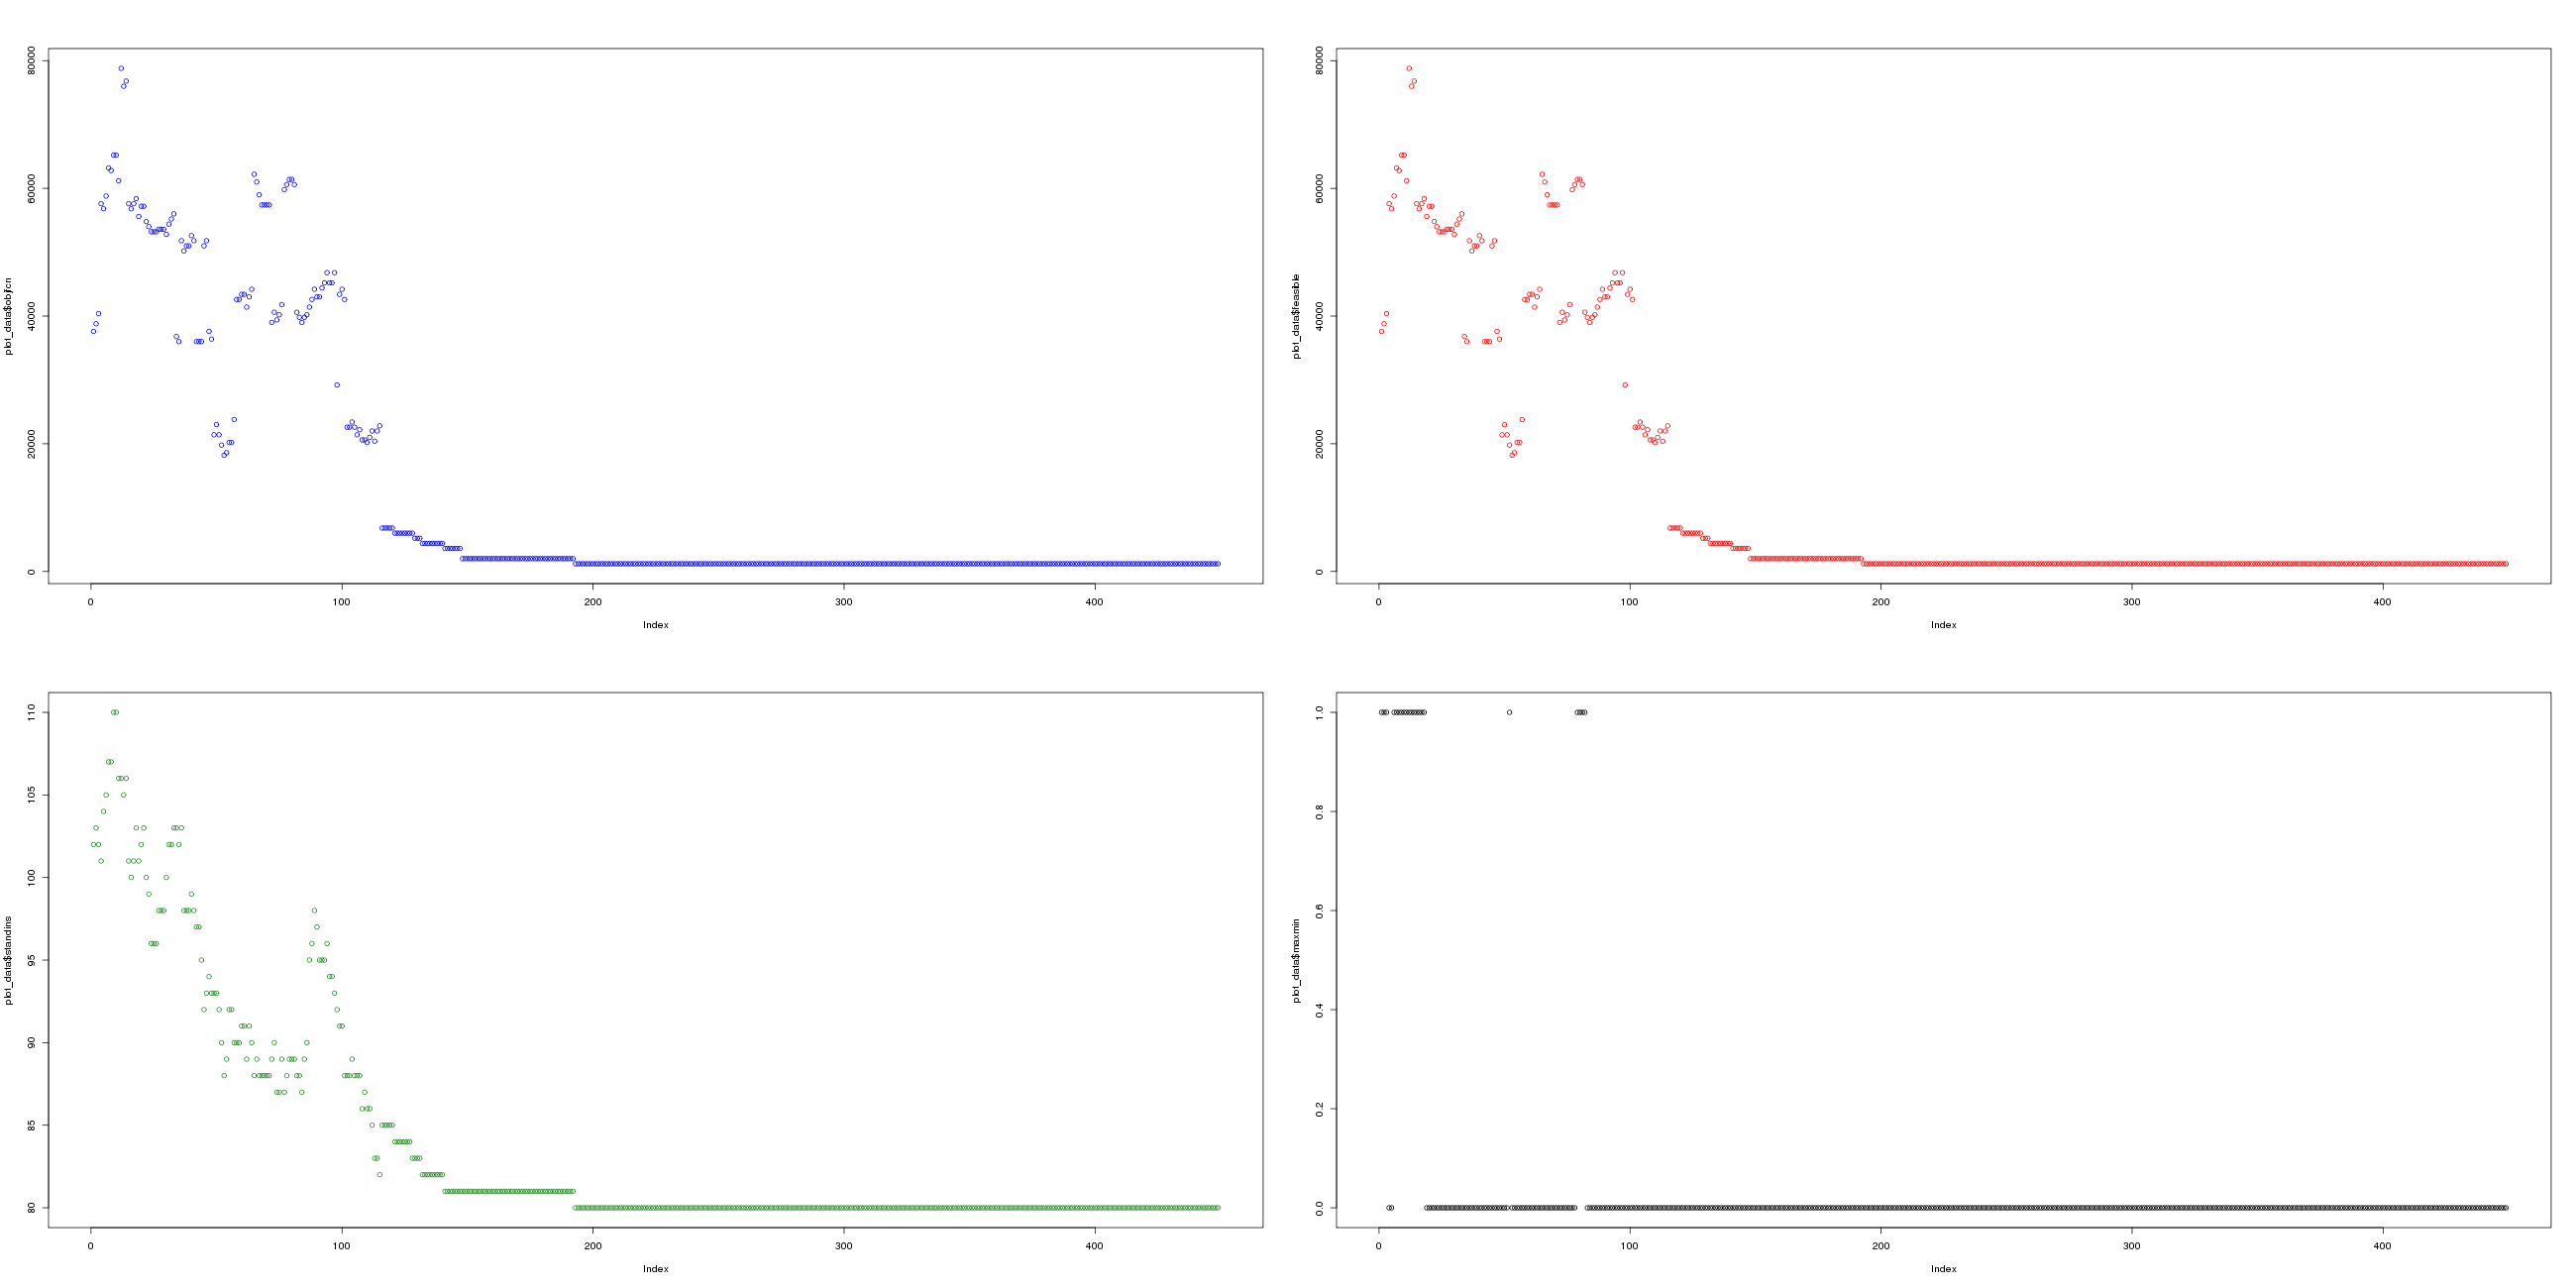
\includegraphics[scale = 0.3, width = 15cm]{Rplot}
%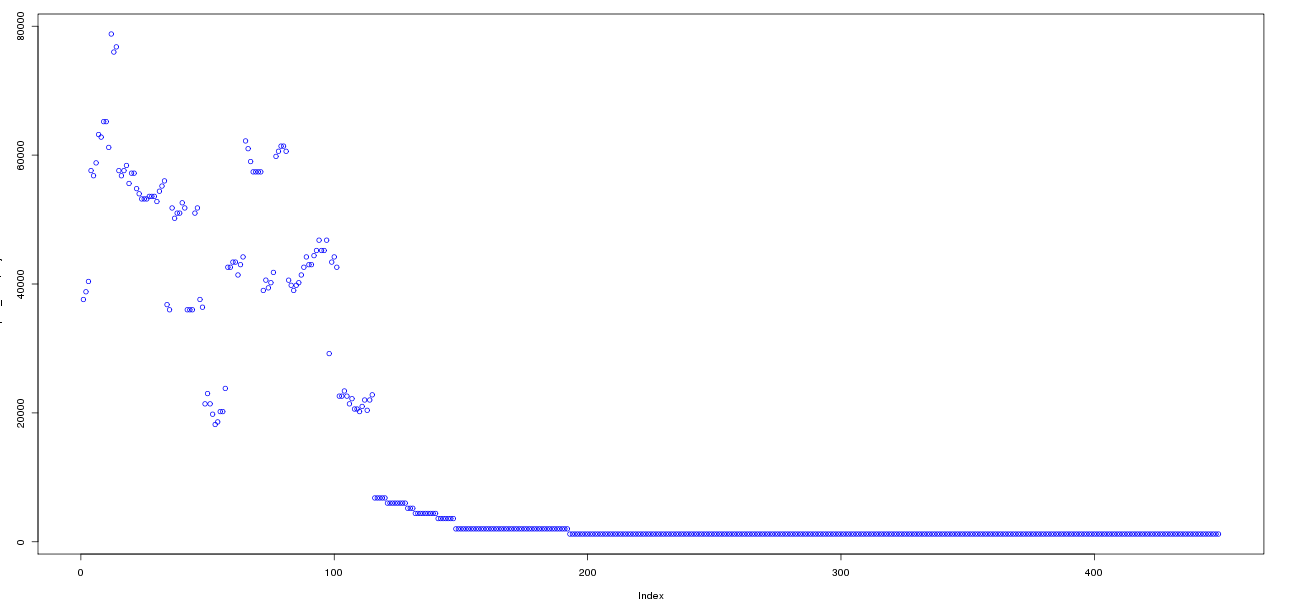
\includegraphics[scale = 0.3, width = 15cm]{1Plot}
\subsection{Task distribution approach}

Some parameter tuning was done in order to find the optimal settings for the algorithm, particularly for the weekend objective function weights described in Section \ref{section:tasks_cost}. The tuning landed in the following parameters
 
Number of iterations, first phase.
Number of iterations, second phase.
$T_0$, $\alpha$
=======
\subsection{Task distribution approach}\label{sec:task_dist_res}

In order to decide the weights described in Section \ref{section:tasks_cost}, different tuning tests were performed. These tests resulted in the weights presented in Table \ref{tab:tasks_weight}. 

\begin{table}[!h]
\centering
\caption{Weights used in the implementation.}
\label{tab:tasks_weight}
\begin{tabular}{|l|l|}
\hline
\rowcolor{Gray} \textbf{Weight} & \textbf{Weight value} \\ \hline
$W_{SI\_m}$ & 0.1 \\ \hline
$W_{S\_m}$ & 0.1 \\ \hline
$W_{D\_m}$ & 10 \\ \hline
$W_{SI\_a}$ & 0.01 \\ \hline
$W_{S\_a}$ & 0.01 \\ \hline
$W_{D\_a}$ & 1 \\ \hline
$W_{w\_SI}$ & 
\begin{tabular} [x]{@{}c@{}}
	2 \text{if librarian} \\ 
	1 \text{if assistant}
\end{tabular} \\ \hline
$W_{Task\_D}$ / $W_{w\_Task\_D}$ & 100\\ \hline
$W_{Task\_W}$ / $W_{w\_Task\_W}$ & 	10 \\ \hline
$W_{PL\_W}$ / $W_{w\_PL\_W}$ & 5 \\ \hline
$W_{PL\_Tot}$ / $W_{w\_PL\_Tot}$ & 5 \\ \hline
$W_{SShift\_W}$ / $W_{w\_SShift\_W}$ & 4 \\ \hline
\end{tabular}
\end{table}

The first six weights, belonging to the weekend objective function, were most experimented with and will be discussed further in this section. The first three have are scaled relatively to each other, while the latter three are simple calculated as one tenth of their equivalent minimum weight. In each of these components, the weights $W_{lib} = 2$ and $W_{ass} = 1$ were used since it can be argued that a librarian can perform twice as many tasks as an assistant.

The individual worker weights and the worker objective function weights are identical in the table since they, relative to each other, decide what soft constraints are most strict. It is, for example more severe to break the rule of one task per day, than to break the rule of having too many shifts at the same time in a week, which is reflected in the weights. Also, in accordance with weights $W_{lib} = 2$ and $W_{ass} = 1$, the stand in cost for librarians is twice the cost of an assistant.

As was argued in Chapter \ref{chap:taskdist}, the critical part of the problem was thought to be the weekend placement part, leading to the implemented two-phase algorithm. Both phases are run a specified number of iterations, referred to as $It_{wend}$ and $It_{wday}$. These parameters were also trimmed and the results from different combination are displayed in Tables \ref{tab:taskdist_res} and \ref{tab:taskdist_weights_res}. 

\begin{table}[!h]
\centering
\label{tab:taskdist_res}
\caption{Results from the task distribution heuristic. Weights form Table \ref{tab:tasks_weight}}
\begin{tabular}{|l|l|l|l|}
\hline
\rowcolor{Gray} \textbf{$It_{wend}/It_{wday}$} &  \textbf{Heuristic cost} &  \textbf{AMPL cost} & \textbf{$\rho_{O\_A}$} \\ \hline
\cellcolor{Gray} \textbf{100/20} & \multicolumn{1}{c|}{5.22} & \multicolumn{1}{c|}{5.48} & 0.58 \\
\cellcolor{Gray} \textbf{500/20} & \multicolumn{1}{c|}{5.64} & \multicolumn{1}{c|}{5.74} & -0.20 \\
\cellcolor{Gray} \textbf{1000/10} & \multicolumn{1}{c|}{5.54} & \multicolumn{1}{c|}{5.66} & 0.03 \\
\cellcolor{Gray} \textbf{1000/20} & \multicolumn{1}{c|}{5.57} & \multicolumn{1}{c|}{5.80} & 0.08 \\
\cellcolor{Gray} \textbf{1000/30} & \multicolumn{1}{c|}{5.50} & \multicolumn{1}{c|}{5.68} & -0.06 \\
\hline
\end{tabular}
\end{table}

\begin{table}[!h]
\centering
\label{tab:taskdist_weights_res}
\caption{Results from the task distribution heuristic when varying weights. All runs with $It_{wend} = 1000$ and $It_{wday} = 20$.}
\begin{tabular}{|l|l|l|}
\hline
\rowcolor{Gray} \textbf{$W_{SI\_m}/W_{S\_m}/W_{D\_m}$} & \textbf{Heuristic cost} &  \textbf{AMPL cost} \\ \hline
\cellcolor{Gray} 0/0/0 & \multicolumn{1}{c|}{2.85} & \multicolumn{1}{c|}{3.66}  \\
\cellcolor{Gray} 1/1/1 & \multicolumn{1}{c|}{5.43} & \multicolumn{1}{c|}{5.54}  \\
\cellcolor{Gray} 10/1/1 & \multicolumn{1}{c|}{5.11} & \multicolumn{1}{c|}{5.36}  \\
\cellcolor{Gray} 1/10/1 & \multicolumn{1}{c|}{5.43} & \multicolumn{1}{c|}{5.60}  \\
\cellcolor{Gray} 1/1/10 & \multicolumn{1}{c|}{5.57} & \multicolumn{1}{c|}{5.80} \\
\hline
\end{tabular}
\end{table}


\begin{figure}[!h]
\centering
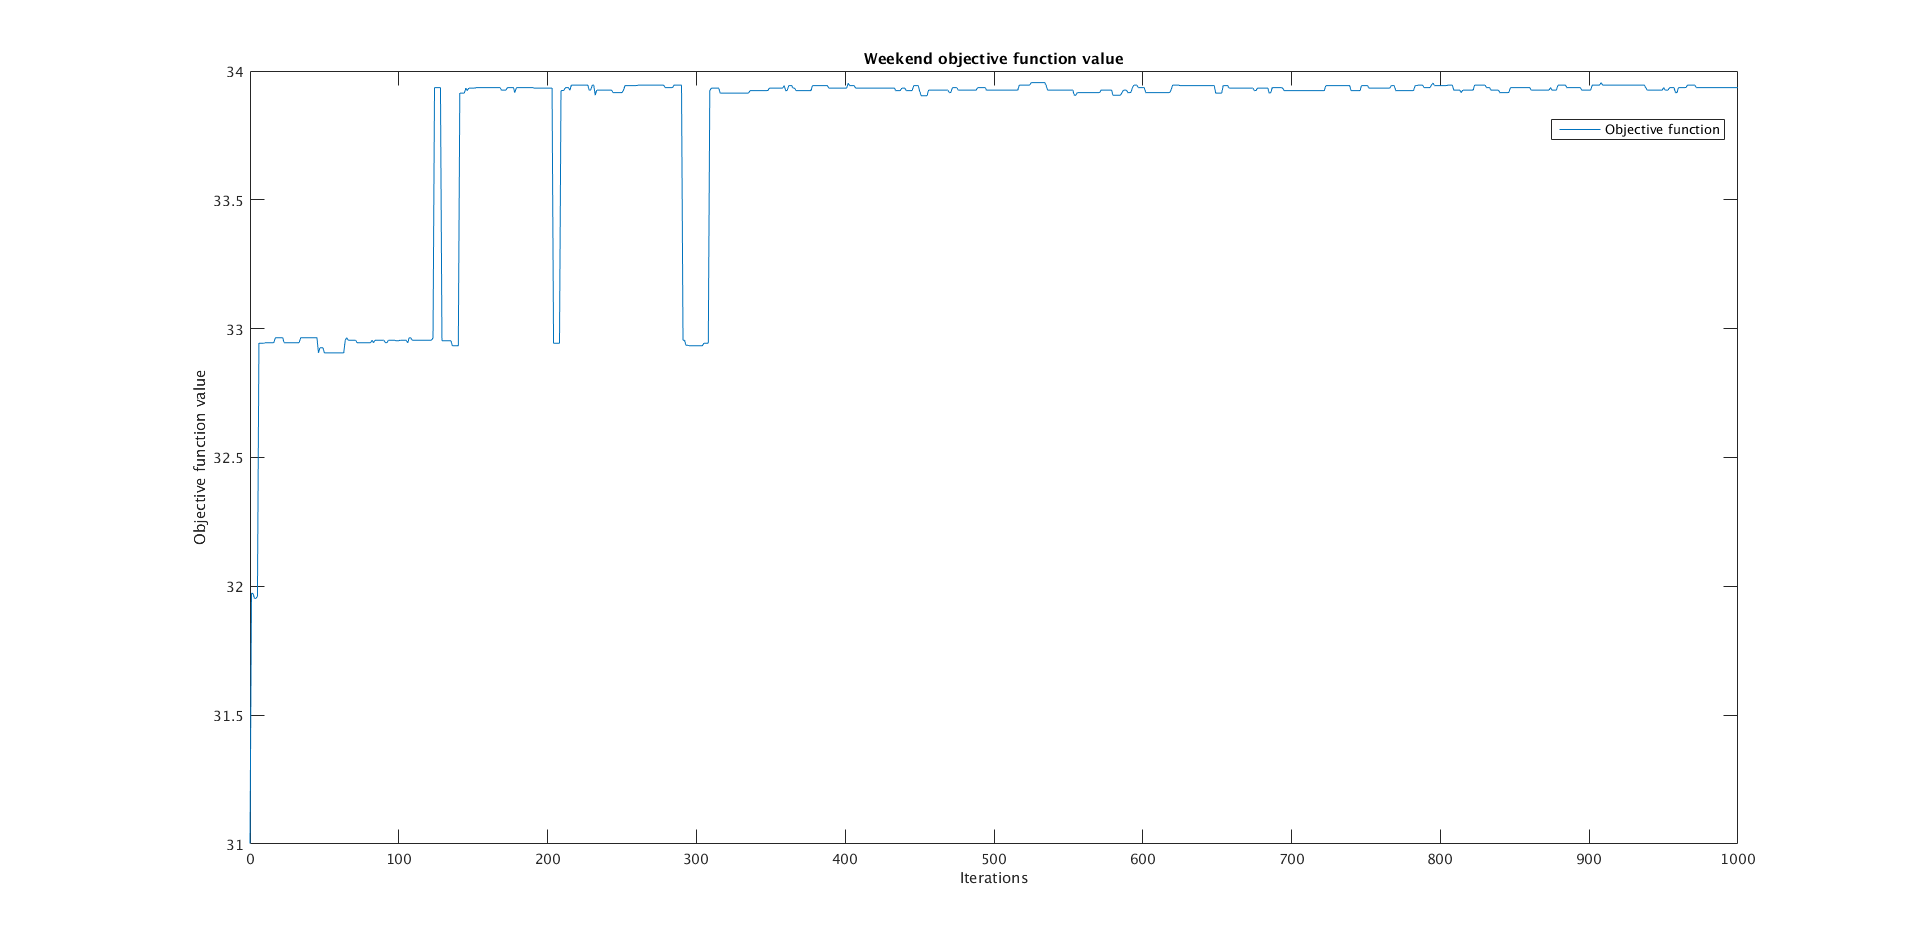
\includegraphics[width=\textwidth, trim = 100px 50px 100px 20px, clip]{Chapters/ImagesEmelie/Plot_1000_20.png}
\caption{Figure of the weekend objective function values for SA parameters $T_0 = 0.4$ and $\alpha = 0.985$. $It_{wend} = 1000$.}
\label{fig:obj_fun_vals}
\end{figure}

The objective function value during a typical run is illustrated by Figure \ref{fig:obj_fun_vals}. The SA accpet function is visible, mainly as a large dive in the objective function value. After about half of the iterations, the SA accepts some deteriorating solutions, but mostly small ones.

>>>>>>> 3acb8311f01de353b66cb667458c31e9680b4aa6

\begin{figure}[!h]
\centering
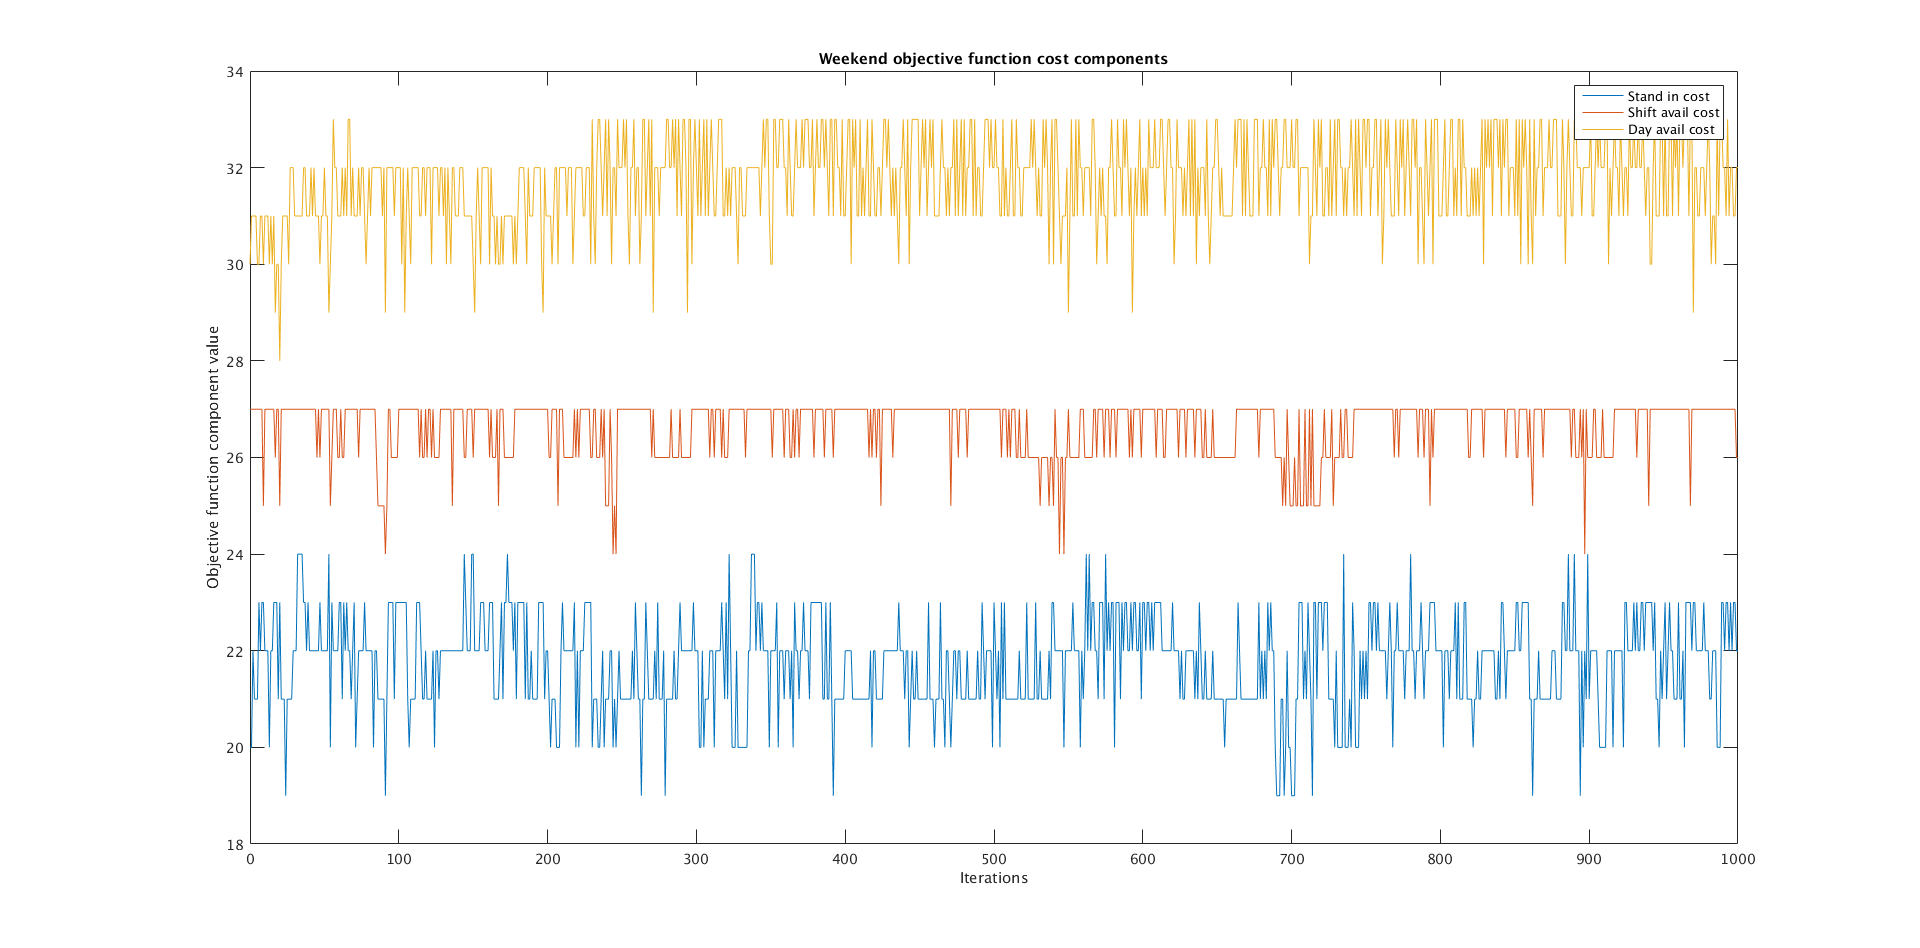
\includegraphics[width=\textwidth, trim = 100px 50px 100px 20px, clip]{Chapters/ImagesEmelie/Components_1000_20.png}
\caption{Figure of the weekend objective minimum costs for SA parameters $T_0 = 0.4$ and $\alpha = 0.985$. $It_{wend} = 1000$.}
\label{fig:obj_fun_comp}
\end{figure}

\begin{figure}[!h]
\centering
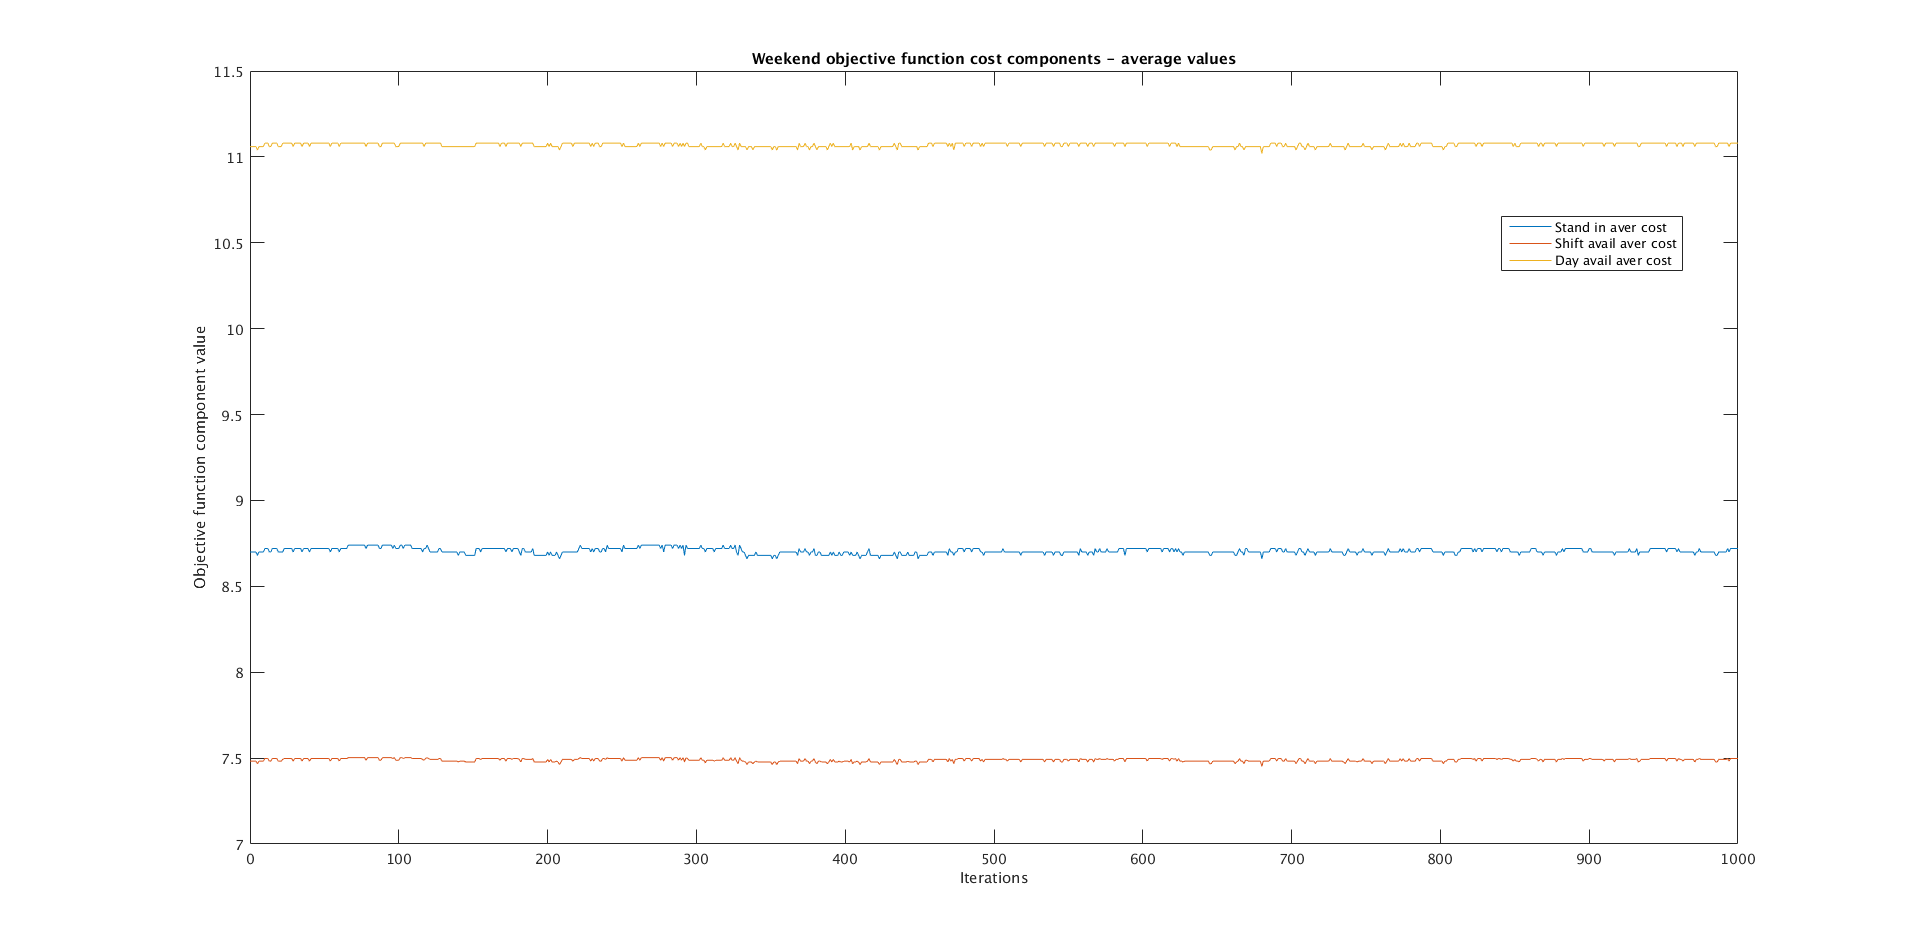
\includegraphics[width=\textwidth, trim = 100px 50px 100px 20px, clip]{Chapters/ImagesEmelie/Components_av_1000_20.png}
\caption{Figure of the weekend objective function average costs for SA parameters $T_0 = 0.4$ and $\alpha = 0.985$. $It_{wend} = 1000$.}
\label{fig:obj_fun_comp_aver}
\end{figure}


In Figure \ref{fig:obj_fun_comp}, the three different min costs from the weekend objective function, without weights, are displayed. Although they seem to constantly vary, a small improvement over iterations can be seen at least in the day avail cost component. Comparing this with Figure \ref{fig:obj_fun_comp_aver}, it can be seen that the average costs do not contribute much to the total objective function value, which is not unexpected.

Correlating the three different variables was done in order to find out if any of the them are interdependent. If that were the case, the choice of weights would be arbitrary. The claculation yielded the following correlation coefficient matrices:

\begin{equation}
  R_{SI\_D} =
  \begin{bmatrix}
 	 1  &  -0.0427 \\
 	 -0.0427  &  1
 \end{bmatrix}
\end{equation}

 \begin{equation}
 R_{SI\_S} =
 \begin{bmatrix}
	 1  &  0.1497 \\
	 0.1497  &  1
 \end{bmatrix}
 \end{equation}
 
\begin{equation}
 R_{S\_D} =
 \begin{bmatrix}
	 1  &  0.0863 \\
	 0.0863  &  1
 \end{bmatrix}
 \end{equation} 
 
 This suggests that there is almost no correlation between the cost components since the top right and bottom left values are close to 0 in all three cases. 0 in these coefficients is equivalent to no correlation while -1 and 1 are indicate a linear correlation. 
 
TODO: plots with 10/20/30 wday iterations. Add 4 different weights. (run to Tuesday).
Write about these results. Correlation between objective function value and AMPL result.

\section{Discussion}
Text


\subsection{Weekly scheduling approach}
Table \ref{pros_cons_weekly_scheduling} lists pros and cons with the implemented weekly scheduling approach. Some pros and cons were considered before the heuristic was chosen. Mainly the con concerning the exponential growth was taken into consideration as an estimation of the upper limit of the problem size was done. Also, the pro regarding the same amount of week blocks was taken into consideration, as the heuristic was thought of having firstly a block construction phase and secondly an assignment phase. 

\begin{table}[!h]
\caption{Pros and cons with the implemented weekly scheduling approach}
\label{pros_cons_weekly_scheduling}
\begin{tabularx}{\linewidth}{>{\parskip1ex}X@{\kern4\tabcolsep}>{\parskip1ex}X}
\toprule
\hfil\bfseries Pros
&
\hfil\bfseries Cons
\\\cmidrule(r{3\tabcolsep}){1-1}\cmidrule(l{-\tabcolsep}){2-2}

%% PROS, seperated by empty line or \par
The same amount of week block appearances will exist for five and ten weeks.\par
Quick iterations when destroying and repairing.\par

&

%% CONS, seperated by empty line or \par
Weekends needs to be assigned in a more systematically way in order to achieve reasonable results regarding lowest amount of stand-ins through the days.\par
The amount of unique block appearances grows exponentially in case more task types are added, such as meetings.\par
The solution time can vary considerably as several random generators have been used.\par
A great deal of costs are needed (some correlated), where each of them affects the solution procedure.

\\\bottomrule
\end{tabularx}
\end{table}

 Weekends, solution time and costs are no major issues as they can be avoided by a few smarter implementations. For instance, weekends can be improved by assigning values when each worker is available on a day and from those numbers create an even distribution of possible stand-ins and therefore increase the lowest value of stand-ins through the days. This shall implicitly decrease the solution time as less iterations will be required. However, to always be able to create a pool of week appearances regardless of problem size can easily become a major issue. Just by adding meetings and the assignment of Library on Wheels tasks to the problem makes it grow considerably.
 

\subsection{Task distribution approach}
Discussion: 

Why do the different weekend weights give such different results?
To what extent is the weekend objective function a good measure of a good schedule?
Conclusion: weekend schedule is ESSENTIAL for a good schedule.

Improve SA?

More tests with average weights.

Further development: look more at weekend objective functions.
